\documentclass[12pt]{article}
\usepackage{amsmath}
\usepackage{amssymb}
\usepackage{algorithm}
\usepackage{algorithmicx}
\usepackage{algpseudocode}
\usepackage{caption}
\usepackage{setspace}
\renewcommand{\baselinestretch}{1.5}
\usepackage[margin=1.0in]{geometry}
\usepackage{float}
\usepackage{graphicx}
\graphicspath{{images/}}
\bibliographystyle{IEEEtran}

\def\code#1{\texttt{#1}}

\begin{document}
\title{MAIA: Modulation Classification with Artificial Intellgence Automata \\ Progress Report I}
\author{Cory Nezin}
\maketitle
\section{Abstract}
Wireless modulation classification has been, and continues to be an important engineering problem.  
Sensing and classifying wireless signals is relevant to applications including government spectrum regulation, cognitive radio, and situational awareness in military/adversarial environments.  ~\cite{DBLP:journals/corr/RajendranCFBCGP17}  Deep neural networks have recently achieved impressive performance in classifying audio, images, and video.  The application of neural networks to wireless communication has recently grown in the machine learning community.  Applications include nonlinear channel modeling, learned data encoding, and modulation classification.  ~\cite{DBLP:journals/corr/OSheaH17}  While promising results have been achieved, they have only been implemented on graphics processing units (GPUs) which have relatively large size, weight, power, and latency compared to FPGAs. ~\cite{Nurvitadhi:2017:FBG:3020078.3021740} We propose a general framework for converting computational graphs (a more general term than neural network) bulit in TensorFlow ~\cite{DBLP:journals/corr/AbadiABBCCCDDDG16} into synthesizable VHDL code for implementation on field programmable gate arrays (FPGAs).

In addition to the size, weight, power, and latency advantages offered by FPGA's, they have also drawn attention in deep learning applications for their reconfigurability from large companies like Microsoft.~\cite{Putnam:2014:RFA:2665671.2665678} Google has also recently developed specialized hardware for deep learning performance enhancement in the form of the "Tensor Processing Unit" (TPU).  The TPU was originally planned to be an FPGA when "[Google] saw that the FPGAs of that time were not competitive in performance compared to the GPUs of that time."~\cite{DBLP:journals/corr/JouppiYPPABBBBB17}  

\section{Introduction}
Automatic modulation classification of wireless signals has been of interest in the signal processing community because of possible applications in cognitive radio.  If a transmitter is not known beforehand, a receiver must detect the transmitted signal, demodulate it, and finally decode it in order to communicate.  Modulation identification is a necessary step in demodulation and is therefore of interest.  It is also possible that in adversarial situations, knowledge of the predominant signal modulation can aid a friendly transmitter in avoiding detection, or allow for more targeted jamming techniques against adversaries.

Convolutional neural networks have been demonstrated as superior to classic techniques in modulation classificaiton.  However, even once they are trained, neural networks are computationally intensive and thus require significant time and power to run on general purpose processors.  MAIA is a hardware architecture tailor made to solve the problem of wireless signal modulation classification using neural networks.  We designed and implemented several core components of a convolutional neural network directly in hardware, explicitly pipelining and optimizing where possible.

The core driving factors of our design are latency and size.  Our goal is to design an architecture which has very little delay between raw received IQ samples and modulation decision made, particularly it should be faster than a general purpose processor.  However, we also want to use a relatively small amount of hardware to reduce size, particularly it should be smaller than a GPU.  We chose to prototype all designs on an FPGA, as a modifiable emulation of true custom hardware (ASIC).  We are using a ZedBoard which contains a Z-7020 FPGA with 85K logic cells, 220 DSP slices, and 4.9Mb of block ram and costs about \$135.00 standalone.

\section{Hardware Contributions}
\subsection{Combinational Matrix Multiply}
The $i^{th}$ element of the product of a matrix, $A$, and a vector, $x$ is given by
$$b_i = \sum_{j=1} A_{ij}x_j$$
Algorithmically, this can be computed with the following pseudocode:

\begin{spacing}{1.0}
\begin{algorithm}
\begin{algorithmic}[1]
    \caption{Matrix Multiplication}
    \State{$b \gets 0$}
    \ForAll{i}
        \ForAll{j}
            \State{$ b_i\gets b_i + A_{ij} \times x_j$}
        \EndFor
    \EndFor
\end{algorithmic}
\end{algorithm}
\label{alg:matmul}
\end{spacing}

In fact, this simple algorithm can be simply recreated in hardware description language (HDL) with a few caveats.  Firstly HDL is not sequential, so when a signal is assigned, it is really more like connecting two wires than attaching some value to some place in memory.  

We now provide an example of a component which multiplies by a $3\times5$ matrix.  First in order to create an inner product, we generate a series of multipliers (one for each column of the matrix)

\begin{spacing}{1.0}
\begin{verbatim}
GEN_MULT:
for i in 0 to 4 generate
begin
  MULTX: multiply
    port map (a => a(n), b => b(n), x => x(n) );
END GENERATE GEN_MULT;
\end{verbatim}
\end{spacing}

Then we add the result of each multiplier up
\begin{spacing}{1.0} \begin{verbatim}
for n in 0 to 4 loop
    s <= s + t(n);
end loop;
x <= s
\end{verbatim} \end{spacing}

Finally to create an entire matrix multiplication, we generate a series of inner products

\begin{spacing}{1.0} \begin{verbatim}
GEN_IP: 
for i in 0 to 2 generate
begin
ip: inner_product
  port map (a => A(i), x => x, b => b(i));
END GENERATE GEN_IP;
\end{verbatim} \end{spacing}

A functional block diagram of the first inner product is shown in figure \ref{fig:naive_inner_product}

\begin{figure}[H]
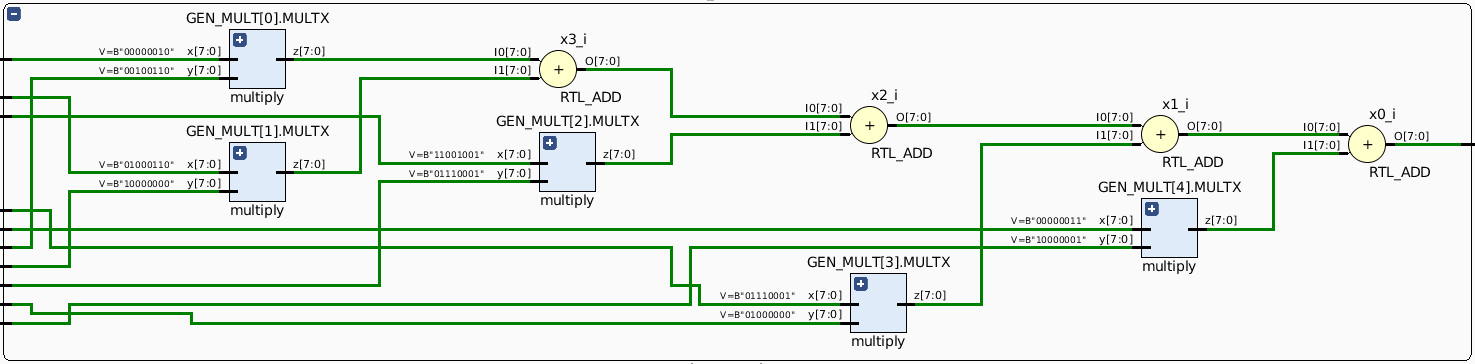
\includegraphics[width=\textwidth]{innerproduct.png}
\caption{A naive implementation of an inner product}
\label{fig:naive_inner_product}
\centering
\end{figure}

The naive construction would produce an output in one clock cycle, giving an extremely good latency.  However it is only feasible for relatively small matrices.  In the neural net architecture chosen for MAIA, matrix multiplication represents about half of the trainable parameters, about $150,000$ coefficients.  The naive implementation would require one DSP slice per parameter, but only 220 DSP slices are available for us to use.  We have not even talked about convolution which makes up the other half of trainable parameters.  It is clear then, that for our large scale problem, we must turn to time domain multiplexing of the hardware.  That is, one matrix multiply must be accomplished over the time frame of many clock cycles, with each DSP slice performing multiple different multiplications.








\subsection{Pipelined Matrix Multiply}
If we look back at algorithm \ref{alg:matmul}, we may see that it is both embarrasingly parallel in that each of the loops with constant $i$ are totally independent.  Furthermore, the only computation is in the form of a multiply-accumulate operation which is an operation which FPGA hardware is already optimized for, and only requires one DSP slice.  So we may allocate some number of DSP slices to process the same number of inner products simultaneously.  Now, the Xilinx DSP48 slice is a fairly complicated component, and we do not require all of its functionality to accomplish this relatively simple task.  In order to simplify our design, we used one of Xilinx's IP cores, the Multiply Adder.  This component essentially provides multiply accumulate functionality in a simple package, the functional block diagram is shown in figure \ref{fig:mac}

\begin{figure}[H]
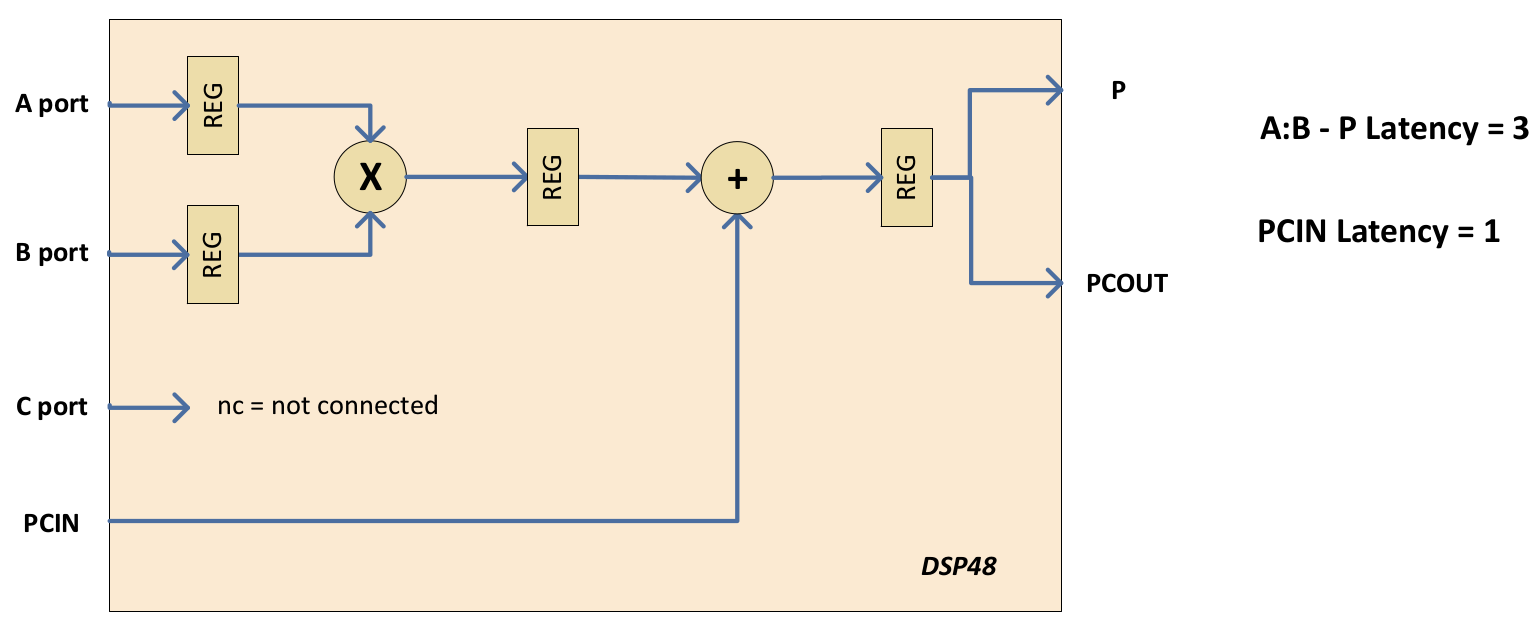
\includegraphics[width=\textwidth]{mac.png}
\caption{Functional diagram of the Multiply Adder}
\label{fig:mac}
\centering
\end{figure}

Connecting the output carry (PCOUT) to the output carry (PCIN) gives a multiply accumulate effect.  Note, however that the latency of the final output is now proportional to the size of the matrix.  More columns means the component will have to accumulate for a longer period of time.  If the amount of rows grows larger than the number of DSP slices we have, which is likely, the rows must be processed in sequence.  To allow for this, we also included a `programmable' state machine in our inner product component which clears the carry after a number of clock cycles indicated by an input signal.

We implemented the design and verified it for a simple test case of two vectors, as shown in figure \ref{fig:inner_product_verify}

\begin{figure}[H]
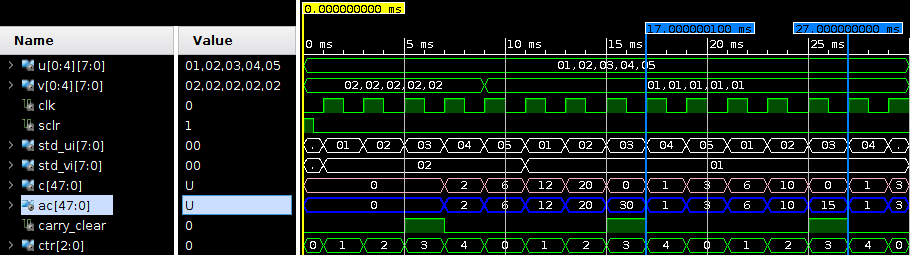
\includegraphics[width=\textwidth]{inner_product_verify.png}
\caption{The waveform of a simple inner product test.}
\label{fig:inner_product_verify}
\centering
\end{figure}

Note the delay of three clock cycles between the final input of the first vector and the final, correct value at the output of the inner product component, \verb|ac|.  The \verb|carry_clear| signal shown is driven by the programmable state machine, which is essentially just creating a signal with a period of 5 clock cycles, the length of the vectors being multiplied.  We will see that this design is useful for not only matrix multiplication, but convolution as well.





\subsection{Systolic Convolution}
Convolution, though it may not seem intuitive, is just a special case of matrix multiplication.  However, the structure of the equivalent matrix is of special structure (Toeplitz) and is usually sparse, which allows for more efficient implementations than regular matrix multiplication.  For instance, an FIR filter can be realized with the direct form, shown in figure \ref{fig:df1}

\begin{figure}[H]
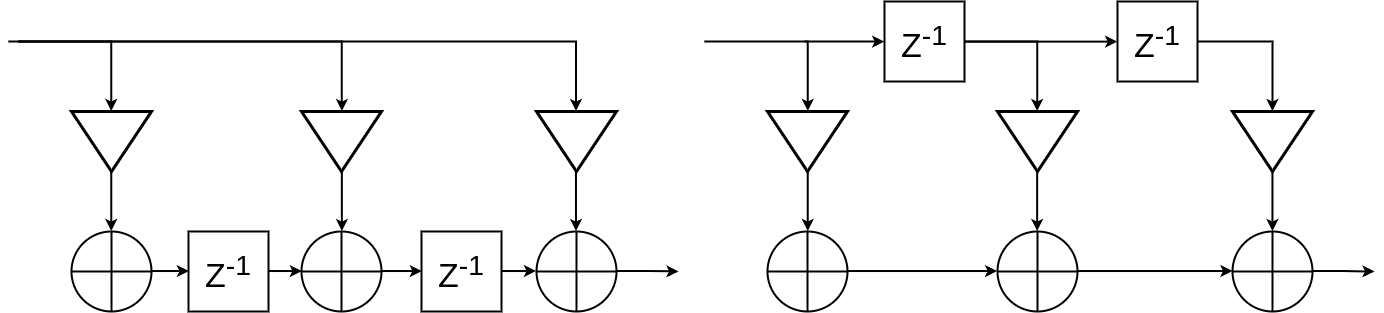
\includegraphics[width=\textwidth]{fir.png}
\caption{Direct Form Transposed (left) and Direct Form (right)}
\label{fig:df1}
\centering
\end{figure}

However, it is clear that if this is actually implemented in hardware, the critical path consists of one multiply and $N$ adders, where $N$ is the length of the filter.  One simple modification, using an adder tree as opposed to an adder chain, would reduce the the critical path to one multiply and $\log_2N$ adders.  However, the direct form transposed, also shown in figure \ref{fig:df1} has a critical path consisting of one multiply and one add, no matter the size of the filter.

Now, each of the multiplies pictured theoretically do not change during the operation of the neural net, so we considered using multiplierless multipliers combined with canonic signed digit represntation for efficient multiplication and filtering.  However, 256 8-tap filters are required for the first convolution stage, meaning we need 2048 multiplies.  However we only have $53,200$ LUTS, and each multiplierless multiplier would require at least 50 LUTS making the design infeasible.  Instead we again turn to time domain multiplexing of the hardware.

Using Xilinx's FIR filter IP core and a controller of our own design, we implemented a component which given a fixed size of data sequentially processes it through each available filter.  This was accomplished by implementing a hybrid queue/circular queue.  First the queue is loaded with samples until full, then whenever a sample is popped from the queue, is broadcast to both the filter and the input of the queue.  This allows the data to repeat for arbitrarily long and so it can be fed through each filter.  The circular queue is a common design pattern in our project since neural nets often have large data parallelism in the form of multiple instruction single data (MISD)

  In the first stage of the neural net, the in-phase and quadrature components of the data are independently filtered with 128 sets of coefficients and then added together.  In order to accomplish this, we instantiated two of the afforementioned components and simply added the result.  We wrote a Python script which verified that the results were correct within error due to fininte precision rounding.

\subsection{Serial Convolution}
Systolic convolution is extremely speed efficient, and relatively simple to implement since IP cores are available directly from Xilinx.  However it is also relatively space inefficient, requiring one DSP slice per tap.  In our original design, we had a misconception regarding the filtering operation in the second stage of the convolution, we beleived that it required 64 16-tap filters.  However, we recently discovered that the nueral net was actually performing essentially a 2D convolution, and we need 128 2D filters consisting of $64\times 16$ kernels.  One could also think of this as $128\times 64$ 16-tap filters.  This would require 8192 16-tap filters.  The FIR filter IP core only allows switching of up to 256 coefficient sets, which means we would have to use 512 DSP slices to accomplish this convolution in a systolic way, significantly more resources than we have.  Therefore we designed the second convolution layer directly with multiply accumulates, similar to the matrix multiplication method already discussed.
The 2D convolution algorithm specific to our case is given in algorithm \ref{alg:conv}, note that $X$ is the output of the previous stage.\\


\begin{spacing}{1.0}
\begin{algorithm}
\begin{algorithmic}[1]
    \caption{2D Convolution}
    \For{$i < 128$} \
        \For{$j < 45$}
            \State{ $s \gets 0$ }
            \State{ $x \gets X[i,j:j+16]$ }
            \For{$k < 16$}
                \State{$ s \gets s + x[k] \times h[15-k]$}
            \EndFor
            \State{$output[i,j] \gets output[i,j] + s$}
        \EndFor
    \EndFor
\end{algorithmic}
\end{algorithm}
\label{alg:conv}
\end{spacing}

Although this is quite abstract and not necessarily easy to map to hardware, we can see that only one multiply accumulator, and therefore one DSP slice is required to perform this operation.  However, it also involves a possibly complex memory access pattern for reading and writing.  To simplify the design, we plan on using circular queues for both reading and writing.  Note that the position that an output is written to is periodic.  If we think of each row in the output matrix as a circular queue, we can simply accumulate s, add it the location in that queue, increment $j$ and shift the queue over one, ready to receive the next `piece' of the output.  The input, $X$ obeys a similar pattern.  Once the first row of samples in $X$ is used, it is never needed again, so we may think of it as a regular queue rather than a circular one.

Note also that line 6, which composes the vast majority of computation is a multiply accumulate operation for vectors of length 16, which represent the signal and the impulse reponse.  Here we can use the inner product component which was already designed for matrix multiplication, since it was designed to accomodate arbitrary vector lengths.  The queue controller has already been designed and is currently being implemented and verified.

\subsection{Max Pooling}
Max pooling is a data dimensionality reduction technique where adjacent samples are compared and only the greater one is kept.  Max pooling in general has two parameters, how many numbers are being compared (the size of the pool) and how far the pool moves between consecutive output samples.  Taking the maximum sample can be viewed as a type of non-linear filtering, the stride can be directly viewed as downsampling.  In the case of our architecture, the downsampling factor is always two, and the pool size is two as well.  Both the conceptual block diagram and the function block diagram are shown in figure \ref{fig:maxpool}

\begin{figure}[H]
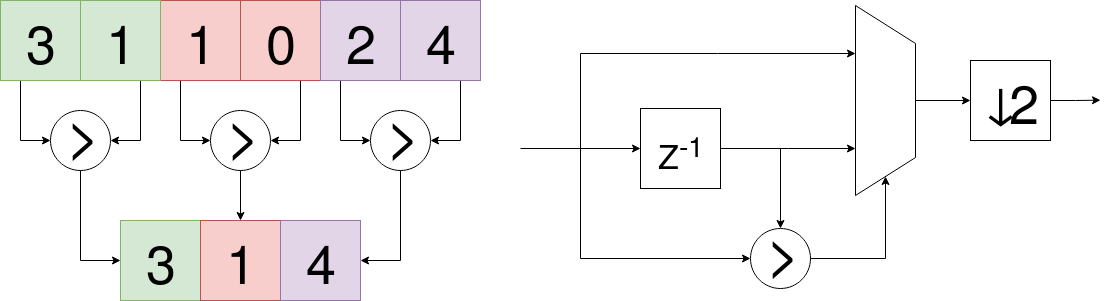
\includegraphics[width=\textwidth]{maxpool.png}
\caption{A naive/conceptual max pool (left) and a pipelined max pool (right) }
\label{fig:maxpool}
\centering
\end{figure}

The actual implementation structure of the max pooling mimics that of an FIR filter.  The difference being addition of adjacent samples has been replaced with a non-linearity, in this case a mux that choses the output based on a comparison of the two samples.  The downsampling block was implemented fairly trivially in raw VHDL.  It is essentially just a clock frequency divider, and so the data rate at all of the following stages is divided by two.  The maxpool unit was exhaustively verified by using a linear feedback shift register (LFSR) to generate every possible pair of samples possible.  The output of the hardware simulation was compared to a simple software implementation and no differences were found.

\subsection{Arg Max}
Arg Max, or arguments of the maxima, are the inputs at which a function or sequence takes on a maximum value.  It can be seen as a special case of max pooling where the pool size and stride are equal to the length of the signal of interest.  In our implementation of the neural net architecture, we deviated here.  The architecture includes what is called a `Softmax' (which is short for soft arg max) function at the very end of the neural net which maps the output of the previous stage to a vector of elements in $(0,1)^{10}$ which represents the neural net's `confidence' about a given modulation scheme.  This is done using sums and quotients of exponential functions, which are very numerically unstable, especially for fixed point.  We chose to do away with this stage and instead replace it with an arg max.  Since softmax preserves ordering, a simple arg max will result in the same decision being made, it doesn't hurt performance at all.  Currently the design and implementation is a farily naive combinational one which was automatically generated by Vivado.  However, the output has been tested and correctly gives the maximum input.  A sample result is shown in figure \ref{fig:argmax}

\begin{figure}[H]
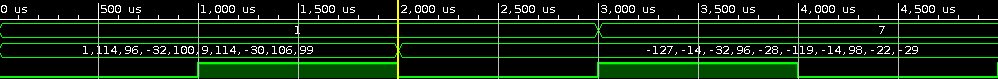
\includegraphics[width=\textwidth]{argmax.png}
\caption{Example output of arg max}
\label{fig:argmax}
\centering
\end{figure}


\section{Conclusion}
The primary components of the neural net have all been designed, and most have been implemented.  Near future work will include finishing the implementation of the serial convolution layer, finishing parallelized matrix multiplication, and connecting the rest of the layers.  Work must also be done in setting up the radio module for the FPGA, however we have encountered setbacks since the most recent software for the radio module is only compaitive with older version of Vivado.  We believe at this rate we should at least be able to complete the neural net implementation by the end of the semester.

%\bibliography{mybib}{}
\end{document}
